%%%%%%%%%%%%%%%%%%%%%%%%%%%%%%%%%%%%%%%%%%%
%
% From a template maintained at https://github.com/jamesrobertlloyd/cbl-tikz-poster
%
%%%%%%%%%%%%%%%%%%%%%%%%%%%%%%%%%%%%%%%%%%%

\documentclass[portrait,a0b,final,a4resizeable]{a0poster}
\setlength{\paperwidth}{36in} % A0 width: 46.8in
\setlength{\paperheight}{48in} % A0 width: 46.8in

\usepackage{qrcode}
\usepackage{multicol}
\usepackage{enumitem}
%\usepackage{color}
%\usepackage{morefloats}
%\usepackage[pdftex]{graphicx}
%\usepackage{rotating}
\usepackage{amsmath, amsthm, amssymb, bm}
%\usepackage{array}
%\usepackage{booktabs}
\usepackage{multirow}
%\usepackage{hyperref}
\usepackage{tikz}
\usetikzlibrary{shapes.geometric,arrows,chains,matrix,positioning,scopes,calc}
\tikzstyle{mybox} = [draw=white, rectangle]
%\definecolor{darkblue}{rgb}{0,0.08,0.45}
%\definecolor{blue}{rgb}{0,0,1}
%\usepackage{dsfont}
\usepackage[margin=0.5in]{geometry}
%\usepackage{fp}

%%%%%%%%%%%%%%%%%%%%%%%%%%%%%%%%%%%%%%%%%%%
%
% myfig
%
% \myfig - replacement for \figure
% necessary, since in multicol-environment
% \figure won't work
%
%%%%%%%%%%%%%%%%%%%%%%%%%%%%%%%%%%%%%%%%%%%

\newcommand{\myfig}[3][0]{
\begin{center}
    \vspace{1.5cm}
    \includegraphics[width=#3\hsize,angle=#1]{#2}
    \nobreak\medskip
\end{center}}

%%%%%%%%%%%%%%%%%%%%%%%%%%%%%%%%%%%%%%%%%%%
%
% mycaption
%
% \mycaption - replacement for \caption
% necessary, since in multicol-environment \figure and
% therefore \caption won't work
%
%%%%%%%%%%%%%%%%%%%%%%%%%%%%%%%%%%%%%%%%%%%

%\newcounter{figure}
\setcounter{figure}{1}
\newcommand{\mycaption}[1]{
\vspace{0.5cm}
\begin{quote}
{{\sc Figure} \arabic{figure}: #1}
\end{quote}
\vspace{1cm}
\stepcounter{figure}
}

%%%%%%%%%%%%%%%%%%%%%%%%%%%%%%%%%%%%%%%%%%%
%
% Some standard colours
%
%%%%%%%%%%%%%%%%%%%%%%%%%%%%%%%%%%%%%%%%%%%

\definecolor{camlightblue}{rgb}{0.601 , 0.8, 1}
\definecolor{camdarkblue}{rgb}{0, 0.203, 0.402}
\definecolor{camred}{rgb}{1, 0.203, 0}
\definecolor{camyellow}{rgb}{1, 0.8, 0}
\definecolor{lightblue}{rgb}{0, 0, 0.80}
\definecolor{white}{rgb}{1, 1, 1}
\definecolor{whiteblue}{rgb}{0.80, 0.80, 1}

%%%%%%%%%%%%%%%%%%%%%%%%%%%%%%%%%%%%%%%%%%%
%
% Some look and feel definitions
%
%%%%%%%%%%%%%%%%%%%%%%%%%%%%%%%%%%%%%%%%%%%

\setlength{\columnsep}{0.03\textwidth}
\setlength{\columnseprule}{0.0018\textwidth}
\setlength{\parindent}{0.0cm}

%%%%%%%%%%%%%%%%%%%%%%%%%%%%%%%%%%%%%%%%%%%
%
% \mysection - replacement for \section*
%
% Puts a pretty box around some text
% TODO - any other thoughts for what this box should look like
%
%%%%%%%%%%%%%%%%%%%%%%%%%%%%%%%%%%%%%%%%%%%

\tikzstyle{mysection} = [rectangle,
draw=none,
shade,
outer color=camlightblue!30,
inner color=camlightblue!30,
text width=0.965\columnwidth,
text centered,
rounded corners=20pt,
minimum height=0.09\columnwidth]

\newcommand{\mysection}[1]
{
\begin{center}
    \begin{tikzpicture}
        \node[mysection] {\sffamily\bfseries\LARGE#1};
    \end{tikzpicture}
\end{center}
}

%%%%%%%%%%%%%%%%%%%%%%%%%%%%%%%%%%%%%%%%%%%
%
% Set the font
%
% TODO - Not sure what a canonical choice is - feel free to modify
%
%%%%%%%%%%%%%%%%%%%%%%%%%%%%%%%%%%%%%%%%%%%

\renewcommand{\familydefault}{cmss}
\sffamily

%%%%%%%%%%%%%%%%%%%%%%%%%%%%%%%%%%%%%%%%%%%%%%%%%%%%
%%%               Background                     %%%
%%%%%%%%%%%%%%%%%%%%%%%%%%%%%%%%%%%%%%%%%%%%%%%%%%%%

\newcommand{\background}[3]{
%\definecolor{cgradbegin}{#1}
%\definecolor{cgradend}{#2}
% \psframe[fillstyle=gradient,gradend=cgradend,
% gradbegin=cgradbegin,gradmidpoint=#3](0.,0.)(1.\textwidth,-1.\textheight)
}




%%%%%%%%%%%%%%%%%%%%%%%%%%%%%%%%%%%%%%%%%%%%%%%%%%%%
%%%                pcolumn                       %%%
%%%%%%%%%%%%%%%%%%%%%%%%%%%%%%%%%%%%%%%%%%%%%%%%%%%%

\newenvironment{pcolumn}[1]{
\begin{minipage}{#1\textwidth}
\begin{center}
}{
\end{center}
\end{minipage}
}



%%%%%%%%%%%%%%%%%%%%%%%%%%%%%%%%%%%%%%%%%%%%%%%%%%%%
%%%                pbox                          %%%
%%%%%%%%%%%%%%%%%%%%%%%%%%%%%%%%%%%%%%%%%%%%%%%%%%%%

\definecolor{lcolor}{rgb}{0, 0, 0.80}
\definecolor{gcolor1}{rgb}{1, 1, 1}
\definecolor{gcolor2}{rgb}{.80, .80, 1}

% \def\fc{fillcolor}
% \def\getfc #1=#2\par{\def\ffc{#1} \ifx\ffc\fc #2\fi}
% \def\getfillcolor #1,#2\par{\getfc #1\par \getfc #2\par}

%  \newcommand{\psshadowbox}[2]{%[2][magenta]{
%      \fbox{Input arg: #1}
%      \fbox{#1}
%      \fbox {\getfillcolor #1\par}
%      \def\col{\getfillcolor #1\par}

%      \let\coll=\col
%       \coll
%     \colorbox{\col}{#2}
%       \mbox
%   \coloredshadowbox{black}{\coll}{#2}
%   }

\newcommand{\pbox}[4]{
%\psshadowbox[#3]{
%\fbox{
\mbox{
\begin{minipage}[t][#2][t]{#1}
#4
\end{minipage}
}%}
}

%%%%%%%%%%%%%%%%%%%%%%%%%%%%%%%%%%%%%%%%%%%
%
% Poster environment
%
% Centres everything and can be used to define the width of the content
%
%%%%%%%%%%%%%%%%%%%%%%%%%%%%%%%%%%%%%%%%%%%

\newenvironment{poster}{
\begin{center}
\begin{minipage}[c]{\textwidth}
}{
\end{minipage}
\end{center}
}

\def\newarrow{\mbox{\begin{tikzpicture}
\useasboundingbox{(-3pt,-4.5pt) rectangle (19pt,1pt)};
\draw[->] (0,-0.07)--(17pt,-0.07);\end{tikzpicture}}}

%%%%%%%%%%%%%%%%%%%%%%%%%%%%%%%%%%%%%%%%%%%
%
% Bottom box
%
%%%%%%%%%%%%%%%%%%%%%%%%%%%%%%%%%%%%%%%%%%%

\newlength{\bottomboxheight}
\setlength{\bottomboxheight}{0.1\paperheight}

\newcommand{\bottombox}[1]{\vfill
\noindent\colorbox{white}{
\begin{minipage}[c][\bottomboxheight][c]{\textwidth}
\centering
\begin{minipage}{0.9\textwidth}
\vfill{

\fontsizesection\color{black}
#1
}

\end{minipage}
\end{minipage}

}
}

%% Bottom box logo
\newcommand{\bottomboxlogo}[2][width=\textwidth]{
\begin{minipage}[c][\bottomboxheight][c]{0.3\textwidth}
\raggedleft\includegraphics[#1]{#2}
\end{minipage}
}

\newcommand{\bottomboxlogoleft}[2][width=\textwidth]{
\begin{minipage}[l][\bottomboxheight][c]{0.3\textwidth}
\raggedleft\includegraphics[#1]{#2}
\end{minipage}
}

%%%%%%%%%%%%%%%%%%%%%%%%%%%%%%%%%%%%%%%%%%%
%
% Highlighting
%
%%%%%%%%%%%%%%%%%%%%%%%%%%%%%%%%%%%%%%%%%%%

\definecolor{slightgray}{rgb}{0.90, 0.90, 0.90}

\usepackage{soul}
\makeatletter
\def\SOUL@hlpreamble{%
\setul{}{3.0ex}%
\let\SOUL@stcolor\SOUL@hlcolor%
\SOUL@stpreamble%
}
\makeatother

\newcommand{\inline}[1]{%
\begingroup%
\sethlcolor{slightgray}%
\hl{\ttfamily\small #1}%
\endgroup
}

\newcommand{\tinline}[1]{%
\begingroup%
\sethlcolor{slightgray}%
\hl{\ttfamily #1}%
\endgroup
}

%%%%%%%%%%%%%%%%%%%%%%%%%%%%%%%%%%%%%%%%%%%
%
% Kotlin syntax highlighting
%
%%%%%%%%%%%%%%%%%%%%%%%%%%%%%%%%%%%%%%%%%%%

\usepackage[skins,breakable,listings]{tcolorbox}

\usepackage[dvipsnames]{xcolor}
\usepackage[table]{xcolor}
\lstdefinelanguage{kotlin}{
comment=[l]{//},
commentstyle={\color{gray}\ttfamily},
emph={delegate, filter, firstOrNull, forEach, it, lazy, mapNotNull, println, @Repeat, return@},
emphstyle={\color{OrangeRed}},
identifierstyle=\color{black},
keywords={abstract, actual, as, as?, break, by, class, companion, continue, data, do, dynamic, else, enum, expect, false, final, for, fun, get, if, import, in, infix, interface, internal, is, null, object, open, operator, override, package, private, public, return, sealed, set, super, suspend, this, throw, true, try, typealias, val, var, vararg, when, where, while, tailrec, reified},
keywordstyle={\color{blue}\bfseries},
morecomment=[s]{/*}{*/},
morestring=[b]",
morestring=[s]{"""*}{*"""},
ndkeywords={@Deprecated, @JvmField, @JvmName, @JvmOverloads, @JvmStatic, @JvmSynthetic, Array, Byte, Double, Float, Int, Integer, Iterable, Long, Runnable, Short, String},
ndkeywordstyle={\color{BurntOrange}\bfseries},
sensitive=true,
stringstyle={\color{ForestGreen}\ttfamily},
literate={`}{{\char0}}1
}

%%%%%%%%%%%%%%%%%%%%%%%%%%%%%%%%%%%%%%%%%%%
%
% Color boxes
%
%%%%%%%%%%%%%%%%%%%%%%%%%%%%%%%%%%%%%%%%%%%

\tcbset{
enhanced jigsaw,
breakable,
listing only,
boxsep=-1pt,
top=-1pt,
bottom=-0.5pt,
right=-0.5pt,
overlay first={
\node[black!50] (S) at (frame.south) {\Large\ding{34}};
\draw[dashed,black!50] (frame.south west) -- (S) -- (frame.south east);
},
overlay middle={
\node[black!50] (S) at (frame.south) {\Large\ding{34}};
\draw[dashed,black!50] (frame.south west) -- (S) -- (frame.south east);
\node[black!50] (S) at (frame.north) {\Large\ding{34}};
\draw[dashed,black!50] (frame.north west) -- (S) -- (frame.north east);
},
overlay last={
\node[black!50] (S) at (frame.north) {\Large\ding{34}};
\draw[dashed,black!50] (frame.north west) -- (S) -- (frame.north east);
},
before={\par\vspace{10pt}},
after={\par\vspace{\parskip}\noindent}
}

\newtcblisting{kotlinlisting}[1][]{%
width=20.5cm,
left=20pt,
top=5pt,
listing options={
language=kotlin,
basicstyle=\ttfamily\normalsize,
%numberstyle=\footnotesize,
showstringspaces=false,
tabsize=2,
breaklines=true,
numbers=none,
inputencoding=utf8,
escapeinside={(*}{*)},
#1
},
underlay unbroken and first={%
\path[draw=none] (interior.north west) rectangle node[white]{
\includegraphics[width=10mm]{../figures/kotlin_file.png}} ([xshift=-18mm,yshift=-20mm]interior.north west);
}
}

\newtcblisting{pythonlisting}[1][]{
width=17cm,
left=20pt,
top=5pt,
listing options={
language=Python,
basicstyle=\ttfamily\normalsize,
upquote=true,
breaklines=true,
showstringspaces=false,
keywordstyle=\color{blue}\bfseries,
escapeinside={(*}{*)},
#1
},
fonttitle=\ttfamily\small,
underlay unbroken and first={
\path[draw=none] (interior.north west) rectangle node[white]{\includegraphics[width=10mm]{../figures/python_icon.png}} ([xshift=-18mm,yshift=-20mm]interior.north west);
}
}

% Imitate syntax error
\usepackage{ulem}
\makeatletter
\def\uwave{\bgroup \markoverwith{\lower7.5\p@\hbox{\sixly \textcolor{red}{\char58}}}\ULon}
\font\sixly=lasy6 % does not re-load if already loaded, so no memory problem.
\makeatother

\usepackage{tikz}
\usepackage[skins,breakable,listings]{tcolorbox}
\usepackage{pgfplots}
\usepackage{tikz-qtree}
\usepackage{graphicx}

\usepackage{include/preamble}


% Custom notation
\newcommand{\fdeep}{\vf^{(1:L)}}
\newcommand{\flast}{\vf^{(L)}}
\newcommand{\Jx}{J_{\vx \rightarrow \vy}}
\newcommand{\Jxx}{J_{\vx \rightarrow \vy}(\vx)}
\newcommand{\Jy}{J_{\vy \rightarrow \vx}}
\newcommand{\Jyy}{J_{\vy \rightarrow \vx}(\vy)}
\newcommand{\detJyy}{ \left| J_{\vy \rightarrow \vx}(\vy) \right|}

\newcommand\transpose{{\textrm{\tiny{\sf{T}}}}}
\newcommand{\note}[1]{}
\newcommand{\hlinespace}{~\vspace*{-0.15cm}~\\\hline\\\vspace*{0.15cm}}
\newcommand{\embeddingletter}{g}
\newcommand{\bo}{{\sc bo}}
\newcommand{\agp}{Arc \gp}

\newcommand{\D}{\mathcal{D}}
\newcommand{\X}{\mathbf{X}}
\newcommand{\y}{y}
\newcommand{\data} {\X, \y}
\newcommand{\x}{\mathbf{x}}
\newcommand{\f}{\mathit{f}}

\newcommand{\fx}{ f(\mathbf{x}) }
\newcommand{\U}{\mathcal{U}}
\newcommand{\E}{\mathbf{E}}


\newcommand{\bardist}[0]{\hspace{-0.2cm}}

\newlength{\arrowsize}
\pgfarrowsdeclare{biggertip}{biggertip}{
\setlength{\arrowsize}{10pt}
\addtolength{\arrowsize}{2\pgflinewidth}
\pgfarrowsrightextend{0}
\pgfarrowsleftextend{-5\arrowsize}
}{
\setlength{\arrowsize}{1pt}
\addtolength{\arrowsize}{\pgflinewidth}
\pgfpathmoveto{\pgfpoint{-5\arrowsize}{4\arrowsize}}
\pgfpathlineto{\pgfpointorigin}
\pgfpathlineto{\pgfpoint{-5\arrowsize}{-4\arrowsize}}
\pgfusepathqstroke
}


% Custom commmands.

\def\jointspacing{\vspace{0.3in}}

\def\boxwidth{0.21\columnwidth}
\newcommand{\gpdrawbox}[1]{
\setlength\fboxsep{0pt}
\hspace{-0.36in}
\fbox{\hspace{-4mm}
%\includegraphics[width=\boxwidth]{../figures/deep_draws/deep_gp_sample_layer_#1}
\hspace{-4mm}}}

\newcommand{\mappic}[1]{
%\hspace{-0.05in}\includegraphics[width=\boxwidth]{../../figures/seed-0-map/latent_coord_map_layer_#1}
}

\newcommand{\mappiccon}[1]{
%\hspace{-0.05in}\includegraphics[width=\boxwidth]{../../figures/seed-0-map-connected/latent_coord_map_layer_#1}
}

\newcommand{\spectrumpic}[1]{
%\includegraphics[trim=4.5mm 0mm 4mm 3mm, clip, width=0.44\columnwidth]{../figures/spectrum/layer-#1}
}

\newcommand{\feat}{\vh}





\begin{document}
  \begin{poster}
    \vspace{1\baselineskip}   % Add some space at the top of the poster


    %%% Header
    \begin{center}
      \begin{pcolumn}{1.03}
        %%% Title
        \begin{minipage}[c][9cm][c]{0.85\textwidth}
          \begin{center}
          {\veryHuge \textbf{Probabilistic Array Programming on Galois Fields}}\\[10mm]
          {\huge Breandan Considine, Jin Guo, Xujie Si\\[7.5mm]
          }
          \end{center}
        \end{minipage}
      \end{pcolumn}
    \end{center}

    \vspace*{1.5cm}

    \large


    %%%%%%%%%%%%%%%%%%%%%%%%%%%%%%%%%%%%%%%%%%%%%%%%%%%%%%%%%%%%%%%%%%%%%%
    %%% Beginning of Document
    %%%%%%%%%%%%%%%%%%%%%%%%%%%%%%%%%%%%%%%%%%%%%%%%%%%%%%%%%%%%%%%%%%%%%%

    \Large

    \begin{multicols}{2}


      \mysection{Main Idea}

      \vspace*{-1cm}
      \null\hspace*{3cm}\begin{minipage}[c]{0.85\columnwidth}
      \begin{itemize}
        \item Boolean matrices are very useful for simulating automata
        \item XOR, AND are functionally complete logical connectives
        \item We implement sketch-based context-free language synthesis
      \end{itemize}
      \end{minipage}

      \jointspacing

      \mysection{Shape errors}
      \vspace*{-1cm}
      \null\hspace*{3cm}\begin{minipage}[c]{0.85\columnwidth}

      There are three broad strategies for handling array shape errors:
      \begin{itemize}[leftmargin=1in]
        \item Perform type coercion by implicitly broadcasting or reshaping arrays
        \item Raise a runtime error (e.g., \tinline{tf.errors.InvalidArgumentError})
        \item Do not allow programs which can result in a shape error to compile
      \end{itemize}

      In Kotlin$\nabla$, we prefer the last strategy. Consider the following scenario:
      \end{minipage}

\null\hspace*{2cm}\begin{minipage}[c]{0.40\columnwidth}
\begin{pythonlisting}
a = np.array('0 1 2 3 4 5')
b = np.array([6, 7, 8])
c = a + b
\end{pythonlisting}
\end{minipage}
\null\hspace*{2cm}\begin{minipage}[c]{0.45\columnwidth}
\begin{kotlinlisting}
val a = Vector(0, 1, 2, 3, 4, 5)
val b = Vector4(arrayOf(6, 7, 8))
val c = (*\uwave{a +\ b}*)
\end{kotlinlisting}
\end{minipage}

\null\hspace*{3cm}\begin{minipage}[c]{0.85\columnwidth}
Similarly, when the inner dimensions of two matrices do not match:
\end{minipage}

\vspace*{-1cm}
\null\hspace*{2cm}\begin{minipage}[c]{0.40\columnwidth}
\begin{pythonlisting}
d = np.matrix('0 1 2; 3 4 5')
e = np.matrix('6 7; 8 9')
f = d @ e
                          \end{pythonlisting}
      \end{minipage}
      \null\hspace*{2cm}\begin{minipage}[c]{0.42\columnwidth}
                          \begin{kotlinlisting}
val d = Matrix2x3(0, 1, 2, 3, 4, 5)
val e = Matrix2x2(6, 7, 8, 9)
val f = (*\uwave{d *\ e}*)
                          \end{kotlinlisting}
      \end{minipage}

      \null\hspace*{3cm}\begin{minipage}[c]{0.85\columnwidth}
We can detect the presence and location of the error within the editor.
      \end{minipage}


      \jointspacing

      \mysection{Type system}
      \vspace*{-1cm}
      \null\hspace*{2cm}\begin{minipage}[c]{0.90\columnwidth}
      \resizebox{\linewidth}{!}{%
      \begin{tabular}{|c|c|c|c|l|}
        \hline Math & Infix & Prefix & Postfix & Operator Type Signature  \\ \hline
        \begin{tabular}{@{}c@{}}$\mathbf{\mathbf{A}}(\mathbf{\mathbf{B}})$\\$\mathbf{\mathbf{A}}\circ\mathbf{\mathbf{B}}$\end{tabular} & \tinline{a(b)} & & & $($\tinline{a}$:  \mathbb{R}^{\tau}\rightarrow\mathbb{R}^{\pi},~$\tinline{b}$: \mathbb{R}^{\lambda} \rightarrow \mathbb{R}^{\tau}) \rightarrow (\mathbb{R}^{\lambda}\rightarrow \mathbb{R}^{\pi})$ \\ \hline
        $\mathbf{\mathbf{A}}\pm\mathbf{\mathbf{B}}$ &  \begin{tabular}{@{}c@{}}\tinline{a + b}\\\tinline{a - b}\end{tabular} &  \begin{tabular}{@{}c@{}}\tinline{plus(a, b)}\\\tinline{minus(a, b)}\end{tabular} &  & $($\tinline{a}$: \mathbb{R}^{\tau}\rightarrow\mathbb{R}^{\pi},~$\tinline{b}$: \mathbb{R}^{\lambda} \rightarrow \mathbb{R}^{\pi}) \rightarrow (\mathbb{R}^{?}\rightarrow \mathbb{R}^{\pi})$ \\ \hline
        $\mathbf{A}  \mathbf{B}$ & \begin{tabular}{@{}c@{}}\tinline{a * b}\\\tinline{a.times(b)}\end{tabular}    & \tinline{times(a, b)} & & $($\tinline{a}$: \mathbb{R}^{\tau}\rightarrow\mathbb{R}^{m \times n},~$\tinline{b}$: \mathbb{R}^{\lambda}\rightarrow\mathbb{R}^{n \times p})  \rightarrow (\mathbb{R}^{?}\rightarrow\mathbb{R}^{m \times p})$ \\ \hline
        \begin{tabular}{@{}c@{}}$\frac{\mathbf{A}}{\mathbf{B}}$\\$\mathbf{A}\mathbf{B}^{-1}$\end{tabular} & \begin{tabular}{@{}c@{}}\tinline{a / b}\\\tinline{a.div(b)}\end{tabular}     & \tinline{div(a, b)}                                    &                                               & $ ($\tinline{a}$: \mathbb{R}^{\tau}\rightarrow\mathbb{R}^{m \times n},~$\tinline{b}$: \mathbb{R}^{\lambda}\rightarrow\mathbb{R}^{p \times n}) \rightarrow (\mathbb{R}^{?}\rightarrow\mathbb{R}^{m \times p})   $ \\ \hline
        %  $\pm\mathbf{\mathbf{A}}$        &                                         & \begin{tabular}{@{}c@{}}\tinline{-a}\\\tinline{+a}\end{tabular}              & \begin{tabular}{@{}c@{}}\tinline{a.unaryMinus()}\\\tinline{a.unaryPlus()}\end{tabular}    & $          ($\tinline{a}$: \mathbb{R}^{\tau}\rightarrow\mathbb{R}^{\pi}) \rightarrow (\mathbb{R}^{\tau}\rightarrow\mathbb{R}^{\pi})                                 $ \\ \hline
        %  \begin{tabular}{@{}c@{}}sin(a)\\cos(a)\\tan(a)\end{tabular}  &                                         & \begin{tabular}{@{}c@{}}\tinline{sin(a)}\\\tinline{cos(a)}\\\tinline{tan(a)}\end{tabular} & \begin{tabular}{@{}c@{}}\tinline{a.sin()}\\\tinline{a.cos()}\\\tinline{a.tan()}\end{tabular} & $($\tinline{a}$: \mathbb{R}\rightarrow\mathbb{R}) \rightarrow (\mathbb{R}\rightarrow\mathbb{R}) $ \\ \hline
        %  $\ln(\mathbf{A})$ & & \begin{tabular}{@{}c@{}}\tinline{ln(a)}\\\tinline{log(a)}\end{tabular} & \begin{tabular}{@{}c@{}}\tinline{a.ln()}\\\tinline{a.log()}\end{tabular}& $($\tinline{a}$: \mathbb{R}^{\tau}\rightarrow\mathbb{R}^{m \times m}) \rightarrow (\mathbb{R}^{\tau}\rightarrow\mathbb{R}^{m \times m})$ \\ \hline
        $\log_b \mathbf{A}$  & \tinline{a.log(b)} & \tinline{log(a, b)} &  & $($\tinline{a}$: \mathbb{R}^{\tau}\rightarrow\mathbb{R}^{m \times m},~$\tinline{b}$: \mathbb{R}^{\lambda}\rightarrow\mathbb{R}^{m \times m}) \rightarrow (\mathbb{R}^{?}\rightarrow\mathbb{R})$ \\ \hline
        $\mathbf{A}^{b}$  & \tinline{a.pow(b)} & \tinline{pow(a, b)} &  & $($\tinline{a}$: \mathbb{R}^{\tau}\rightarrow\mathbb{R}^{m \times m},~$\tinline{b}$: \mathbb{R}^{\lambda}\rightarrow\mathbb{R}) \rightarrow (\mathbb{R}^{?}\rightarrow\mathbb{R}^{m \times m})$ \\ \hline
        %  \begin{tabular}{@{}c@{}}$\sqrt{a}$\\$\sqrt[3]{a}$\end{tabular} & \begin{tabular}{@{}c@{}}\tinline{a.pow(1.0/2)}\\\tinline{a.root(3)}\end{tabular} & \begin{tabular}{@{}c@{}}\tinline{a.pow(1.0/2)}\\\tinline{a.root(3)}\end{tabular}     & \begin{tabular}{@{}c@{}}\tinline{a.sqrt()}\\\tinline{a.cbrt()}\end{tabular} & $($\tinline{a}$: \mathbb{R}^{\tau}\rightarrow\mathbb{R}^{m \times m}) \rightarrow (\mathbb{R}\rightarrow\mathbb{R}^{m \times m})$ \\ \hline
          \begin{tabular}{@{}c@{}}$\frac{da}{db}$, $\frac{\partial{a}}{\partial{b}}$\\$D_{b}a$\end{tabular} & \begin{tabular}{@{}c@{}}\tinline{a.d(b)}\\\tinline{d(a)/d(b)}\end{tabular}                               & \tinline{grad(a)[b]}                                   &                                    & $          \big($\tinline{a}$: C(\mathbb{R}^{\tau}\rightarrow\mathbb{R}),~$\tinline{b}$: C(\mathbb{R}^{\lambda}\rightarrow\mathbb{R})\big) \rightarrow (\mathbb{R}^{?}\rightarrow\mathbb{R})                          $ \\ \hline
        $\nabla a$  &  & \tinline{grad(a)} & \tinline{a.grad()} & $\big($\tinline{a}$: C(\mathbb{R}^{\tau}\rightarrow\mathbb{R})\big) \rightarrow (\mathbb{R}^{\tau}\rightarrow\mathbb{R}^{\tau})$ \\ \hline
        $\nabla_{\mathbf{B}} a$  & \begin{tabular}{@{}c@{}}\tinline{a.d(b)}\\\tinline{a.grad(b)}\end{tabular} & \tinline{grad(a, b)} &  & $\big($\tinline{a}$: C(\mathbb{R}^{\tau}\rightarrow\mathbb{R}),~$\tinline{b}$: C(\mathbb{R}^{\lambda}\rightarrow\mathbb{R}^{n})\big) \rightarrow (\mathbb{R}^{?}\rightarrow\mathbb{R}^{n})$ \\ \hline
        $\nabla\cdot{\mathbf{A}}$ & & \tinline{divg(a)} & \tinline{a.divg()} & $\big($\tinline{a}$: C(\mathbb{R}^\tau \rightarrow \mathbb{R}^m)\big) \rightarrow (\mathbb{R}^\tau \rightarrow \mathbb{R})$\\ \hline
        $\nabla\times{\mathbf{A}}$ & & \tinline{curl(a)} & \tinline{a.curl()} & $\big($\tinline{a}$: C(\mathbb{R}^3 \rightarrow \mathbb{R}^3)\big) \rightarrow (\mathbb{R}^3 \rightarrow \mathbb{R}^3)$\\ \hline
%        $\mathcal{J}(\mathbf{A})$ & & \tinline{grad(a)} & \tinline{divg(a)} & $\big($\tinline{a}$: C(\mathbb{R}^\tau \rightarrow \mathbb{R}^m)\big) \rightarrow (\mathbb{R}^\tau \rightarrow \mathbb{R}^{m\times\tau})$\\ \hline
%        $\mathcal{J}_{\mathbf{B}}(\mathbf{A})$ & & & & $ \big($\tinline{a}$: C(\mathbb{R}^\tau \rightarrow \mathbb{R}^m),~$\tinline{b}$: C(\mathbb{R}^\lambda \rightarrow \mathbb{R}^n)\big) \rightarrow (\mathbb{R}^{?} \rightarrow \mathbb{R}^{m\times n})$\\ \hline
%        $\mathbf{H}(a)$ & & & & \\ \hline
%        $\Delta{a},\nabla^{2}a$ & & & & \\ \hline
      \end{tabular}
      }
      \end{minipage}

      \jointspacing

      \mysection{Differentiable Programming}

      \null\hspace*{2cm}\begin{minipage}[c]{0.90\columnwidth}\center\resizebox{0.95\linewidth}{!}{\includegraphics{../figures/diff_prob_prog.png}}
      \end{minipage}

      \jointspacing

      \mysection{Visualization}
      \vspace*{-2cm}
%      \null\hspace*{3cm}\begin{minipage}[c]{0.85\columnwidth}Kotlin$\nabla$ is capable of computing arbitrarily high order derivatives.\end{minipage}\\
\null\hspace*{2cm}\begin{minipage}[c]{0.48\columnwidth}
\begin{kotlinlisting}
val y = sin(sin(sin(x))) / x
val z = y + sin(x) * x + cos(x) + x
val d1 = d(z) / d(x)
val d2 = d(d1) / d(x)
val d3 = d(d2) / d(x)
val d4 = d(d3) / d(x)
val d5 = d(d4) / d(x)
plot2D(-6..6, z, d1, d2, d3, d4, d5)
\end{kotlinlisting}
\end{minipage}
    \null\hspace*{2cm}\begin{minipage}[c]{0.40\columnwidth} \vspace*{1.5cm}\center\resizebox{0.95\linewidth}{!}{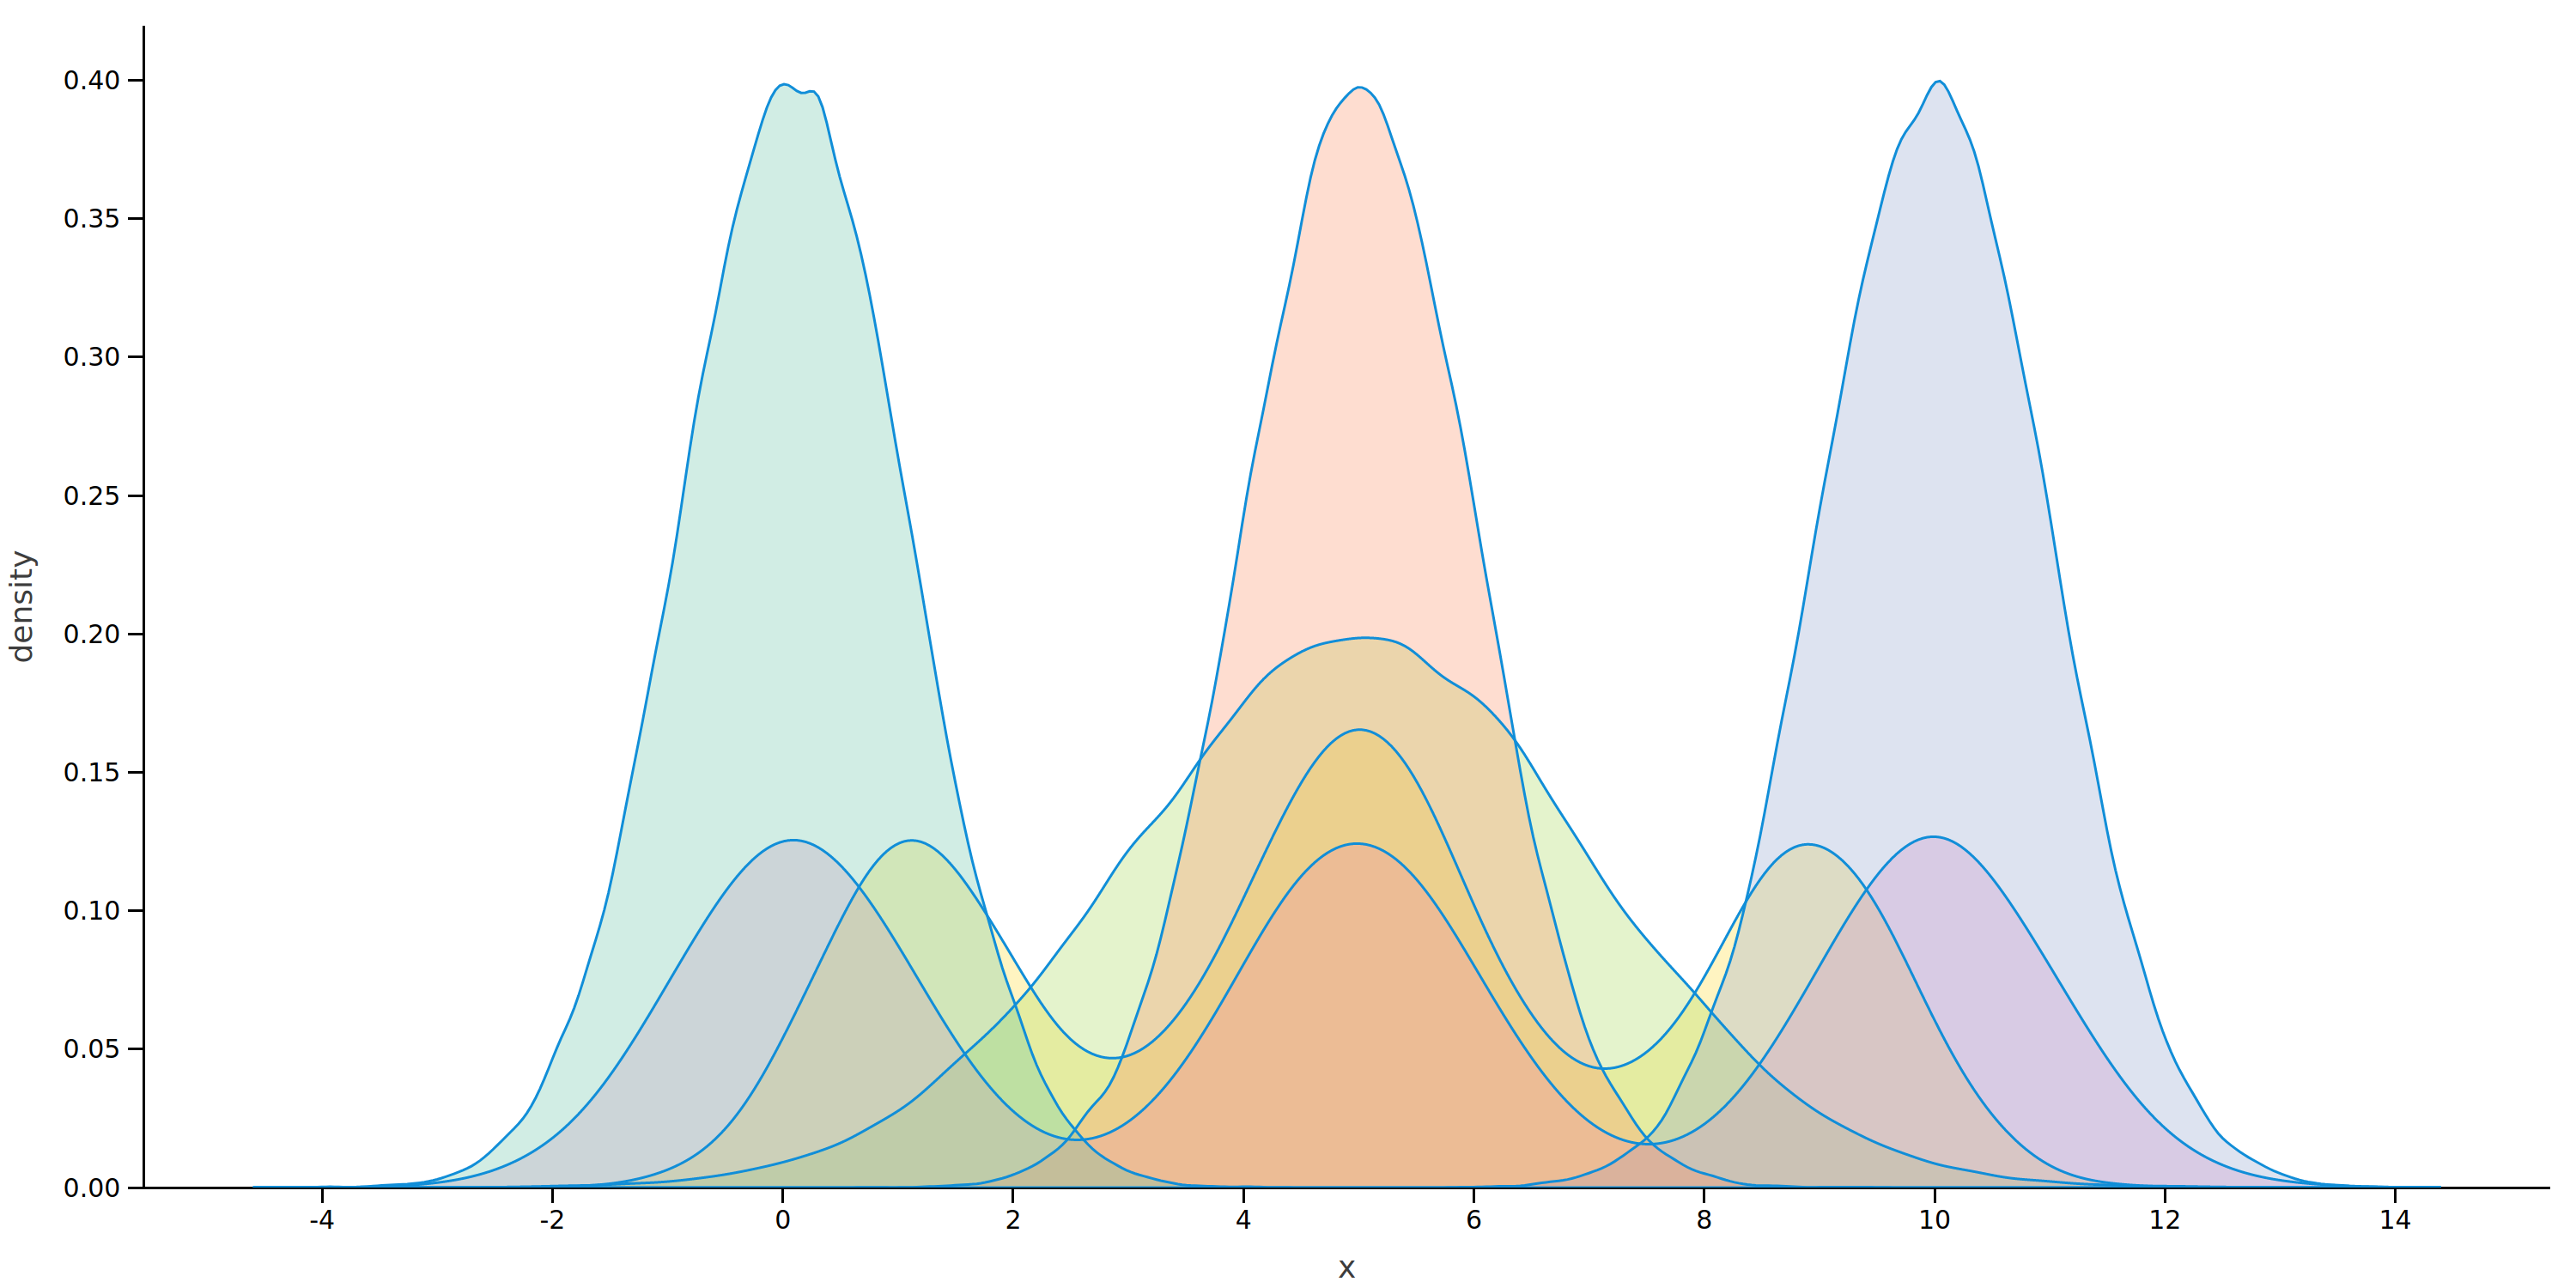
\includegraphics{../figures/plot.png}}\end{minipage}

\null\hspace*{2cm}\begin{minipage}[c]{0.515\columnwidth}
\begin{kotlinlisting}
val Z = x * x + pow(y, 2)
val Z10 = Z * 10
val sinZ = sin(Z10)
val sinZ_10 = sinZ / 10
val dZ_dx = d(sinZ_10) / d(x)
val d2Z_dxdy = d(dZ_dx) / d(y)
val d3Z_d2xdy = d(d2Z_dxdy) / d(x)
plot3D(-1..1, d3Z_d2xdy)
\end{kotlinlisting}
\end{minipage}
      \null\hspace*{2cm}\begin{minipage}[c]{0.30\columnwidth}\center\resizebox{0.95\linewidth}{!}{\includegraphics{../figures/plot3d.png}}\end{minipage}

      \jointspacing


      \mysection{Physical Simulation}

      %      \null\hspace*{3cm}\begin{minipage}[c]{0.85\columnwidth}We simulate a double pendulum described by the following equations:\end{minipage}\\

      \centering
      ${\displaystyle L={\tfrac {1}{6}}ml^{2}\left({{\omega}_{2}}^{2}+4{{\omega}_{1}}^{2}+3{{\omega}_{1}}{{\omega}_{2}}\cos(\theta _{1}-\theta _{2})\right)+{\tfrac {1}{2}}mgl\left(3\cos \theta _{1}+\cos \theta _{2}\right)}$
      ${\displaystyle {\begin{aligned}{{\omega}_{1}}&={\frac {6}{ml^{2}}}{\frac {2p_{\theta _{1}}-3\cos(\theta _{1}-\theta _{2})p_{\theta _{2}}}{16-9\cos ^{2}(\theta _{1}-\theta _{2})}}\\{{\omega}_{2}}&={\frac {6}{ml^{2}}}{\frac {8p_{\theta _{2}}-3\cos(\theta _{1}-\theta _{2})p_{\theta _{1}}}{16-9\cos ^{2}(\theta _{1}-\theta _{2})}}\end{aligned}}}$\\
      ${\displaystyle {\begin{aligned}{{{p}}_{\theta _{1}}}&={\frac {\partial L}{\partial \omega _{1}}}, {{{p}}_{\theta_{2}}}&={\frac {\partial L}{\partial \omega_{2}}}, {{\dot {p}}_{\theta _{1}}}&={\frac {\partial L}{\partial \theta _{1}}}, {{\dot {p}}_{\theta _{2}}}&={\frac {\partial L}{\partial \theta _{2}}}\end{aligned}}}$\\
      \null\hspace*{2cm}\begin{minipage}[c]{0.80\columnwidth}\center\resizebox{0.85\linewidth}{!}{\includegraphics{../figures/double_pendulum.png}}
      \end{minipage}

      \jointspacing

      \mysection{Numerical Precision}

      \begin{tikzpicture}
      \begin{axis}[title={Log errors evaluating $f(x) = \frac{\sin\sin\sin x}{x} + x \sin x + \cos x + x$}, height=20cm, width=35cm, xlabel=$x$, ylabel=$\log_{10}(\Delta)$, xmin=-1000, xmax=1000, xtick={-1000,-750,...,1000}, legend pos=south east, legend style={font=\small}, align=center, compat=newest]
      \addplot table [mark=none, x index=0, y index=1, col sep=comma] {../data/adsd_comparison.csv};
      \addlegendentry{$\Delta$(SD, AP) $\approx\Delta$(AD, IP)}
      \addplot table [mark=none, x index=0, y index=2, col sep=comma] {../data/adsd_comparison.csv};
      \addlegendentry{$\Delta$(AD, SD)}
      \addplot table [mark=none, x index=0, y index=3, col sep=comma] {../data/adsd_comparison.csv};
      \addlegendentry{$\Delta$(FD, AP)}
      \end{axis}
      \end{tikzpicture}
      \jointspacing

    \end{multicols}

    \bottombox{
    %% QR code
    %    \hfill\bottomboxlogo{img/kotlin_logo.png}
    % Comment out the line below out to hide logo
    \begin{minipage}[c][0.1\paperheight][c]{0.2\textwidth}\qrcode[height=3in]{ssnp.ndan.co} \end{minipage}
    \begin{minipage}[c][0.1\paperheight][c]{0.2\textwidth}
\includegraphics[height=3in]{../figures/fpt_logo.png} \end{minipage}
    \begin{minipage}[c][0.1\paperheight][c]{0.33\textwidth}
\includegraphics[height=3in]{../figures/mcgill.png} \end{minipage}
    \begin{minipage}[c][0.1\paperheight][c]{0.33\textwidth}
\includegraphics[height=4in]{../figures/mila.png} \end{minipage}
    %    \hfill\bottomboxlogo{img/mila_mauve.png} % \hfill shifts the logo across so it meets the right hand side margin
    % Note that \bottomboxlogo takes an optional width argument. It defaults to the following:
    % \hfill\bottomboxlogo[width=\textwidth]{<path_to_image_file>}
    % where \textwidth is actually the width of a minipage which is defined in the \bottombox command of
    % betterportaitposter.cls It's a standard \includegraphics command in there, so easy to change if
    % you need to add a border etc.
    }
\end{poster}
\end{document}
